 \chapter[Komunikační bezpečnost]{B4M36KBE \\[1ex]\Large{Zásady návrhu bezpečných systémů. Design a analýza bezpečnosti komunikačních protokolů a komunikačních médií. Bezpečnost distribuovaných systémů.}}
 
Co je bezpečnost? To nejde jednoznačně definovat.
\begin{itemize}
\item need to know (data jsou dostupná právě tomu, komu mají být dostupná)
\item systém je bezpečný, pokud cena jeho prolomení je vyšší než hodnota dat
\item systém je bezpečný, pokud představa uživatelů o bezpečnosti odpovídá realitě
\item dveře od učebny jsou bezpečné, protože sice jdou snadno vykopnout, ale nikdo od nich nečeká víc (tj můžeme jim věřit)
\item pokud se něco tváří bezpečně, ale není, pak to je riziko, protože bezpečnost očekáváme a žádná tam není
\end{itemize}

Bezpečnost (safety): zakopnu o práh dveří, pravděpodobnost je Gaussovská
Bezpečnost (security): zakopnu o provázek, který mi tam někdo zcela záměrně natáhl
 - pokud děláme bezpečnost (security), nemůžeme se bránit proti průměrnému případu, ale proti zcela záměrnému útoku

Bezpečnost se realizuje v několika krocích:
\begin{enumerate}
\item \textbf{Politika} bezpečnosti (na BSY se tomu říkalo směrnice) říká, co a jak se snažíme zabezpečit, jsou to lidsky řečená pravidla (ale měla by být přesná). Týkají se zabezpečení jak uživatelů, tak dat.
\item \textbf{Protokoly} definují, jaké technologie použijeme k dosažení cílů politiky.
\item \textbf{Realizace protokolu} říká např. jaká kryptografie je vhodná.
\end{enumerate}
 
Nejvíc bezpečnostních chyb se děje na rozhraní Protokolů a realizace, protože protokoly mají nějaké předpoklady, které ale realizace často nemá.

\paragraph{Co se snažíme zabezpečit?} Systém je to, co se snažíme zabezpečit, může to být jedno zařízení, nebo celá síť včetně uživatelů. Např. v případě SIM karty nás zajímá karta samotná, vodivé spoje v ní, ochrana proti vniknutí do hardwaru, dále telefon, do kterého kartu strčíme, síť, do které se telefon připojí, a nakonec jsou součástí systému i jeho uživatelé.

Věci uvnitř systému se jmenují následovně:
\begin{description}
\item[subjekt] fyzický člověk, který je někde v systému
\item[person] ne člověk, ale osoba fyzická nebo osoba právnická. Do češtiny se překládá jako "osoba"
\item[principal] někdo/něco, co se účastní komunikace. Pokud řešíme vložení SIM do telefonu, tak principal jsou SIM karta a telefon. Pokud řešíme GSM síť, tak principals jsou telefony v síti a vysílače.
\end{description}

   
CIA:
 - Confidentiality: data jsou tajná a vidí je jen ti, kdo smí. Zkráceně, jde o "povinnost chránit", policy
   - privacy: policy o tom, že/jak budu chránit data
   - secrecy: implementace dané policy
 - Integrity: data můžou měnit jen ti, kdo smí (a podle jasně daných pravidel), data jsou tedy garantovaně správná a můžeme jim věřit
 - Availability: data jsou dostupná (a systém, kde jsou data dostupná, je v použitelném stavu)

šifrování webové stránky (zpravodajství) mezi serverem a prohlížečem slouží k 
privacy chrání osobní údaje, ale ne data firmy (pokud v tom ovšem není nic o zaměstnancích)

Pravidla o privacy se liší mezi různými státy:
 - v Číně na ulici státní kamery monitorují občany
 - v USA naopak stát tyto informace shromažďovat nesmí, můžou to dělat jen soukromníci (asi za nějakých podmínek)
 


 
Anonymita: právo nebýt identifikován
Freshness: nejde o zopakování starší zprávy
Trust: něco, do čeho vkládáme svou bezpečnost
 - trusted: trezor, do kterého dám své cennosti (=věřím mu)
 - trustworthy: trezor, který dokáže moje cennosti ochránit (v češtině je přesný překlad "důvěryhodnost")

Příště: protokoly



Přednáška 2: 
Protokoly

 Důležité pojmy:
 - identifikace: ověření, že jedinec je ten, za koho se vydává
 - autentifikace: ověření, že jedinec patří do nějaké skupiny
 - autorizace: ověření, že jedinec může udělat danou akci


\section{Vývoj protokolů v čase}

\subsection{Vstup do hradu}

Dejme tomu, že chceme zabránit vojákům nepřítele v tom, aby vstoupil do hradu, uděláme to tak, že si dohodneme heslo, a bude to fungovat následovně:
\begin{enumerate}
\item stráž se zeptá na heslo (challenge)
\item vstupující voják odpoví (response/password)
\item stráž se rozhodne (buď vpustit, nebo zabít)
\end{enumerate}

Takový protokol jde napadnout několika způsoby:
\begin{itemize}
\item eavesdropping: za křovím odposlechneme, jak voják říká správné heslo a pak ho zopakujeme stráži
\item rubber hosing: zajmeme nějakého vojáka a gumovou hadicí ho mlátíme, dokud nám heslo neřekne
\item unauthenticated challenge: s uniformou si stoupneme někam, kde žádná stráž není, a ptáme se procházejících vojáků na heslo
\item brute force: jdeme k bráně a tipneme heslo "vítězství", "sláva císaři" atd
\item bribery: podplatíme stráž
\end{itemize}

Hlavní slabiny jsou:
\begin{itemize}
\item heslo se v čase nemění (jde odposlechnout dnes a použít za týden)
\item heslo jde otevřeným kanálem, říká se nahlas a proto jde odposlechnout
heslo je sdílené (všichni vojáci mají stejné jedno heslo)
\end{itemize}

\subsection{Čtečka karet}

Funguje podobně jako vstup do hradu. Rozdíl je v tom, že karta přiložená ke čtečce neřekne heslo, ale nahlásí své číslo. Čtečka pak v databázi zkontroluje, jestli smí karta s tímto číslem otevřít dveře.

Od hradu se zlepšilo to, že každý uživatel má svou kartou s unikátním číslem, takže nejde o sdílené tajemství. Taky je těžší odposlechnout kartu než slovně předané heslo

\subsection{Vrata do garáže}

V první hloupé variantě vrata čekají na klíč. Klíč pošle heslo a nonce (unikátní číslo na jedno použití - nonce N) zašifrované klíčem, které sdílí s garáží. Vrata zprávu dešifrují a musí ověřit, že heslo je správné, a že N nebylo poslední dobou použité. Tentokrát jsou odposlechy těžší, ale visí to na tom, že garáž si pamatuje poslední použitá N. Lepší by bylo, kdyby garáž sama určovala, jaké N se použije.

V lepší variantě vrata pošlou klíči výzvu - nonce. Klíč přidá svoje heslo, zašifruje nonce a pošle ho zpět. Vrata zprávu dešifrují a opět ověří správnost. Bezpečnost v tomto případě visí na tom, že se nonce opravdu použije jen jednou. Je potřeba mít dobře dělaný náhodný generátor, dostatečně velký prostor nonce, používat různé seedy a generátor nesmí jít zvenku resetovat.

\subsection{Auta}

Dálková ovládání od aut mají v sobě klíče, které se generují v továrně na základě VINu. V továrně mají master key, tím se VIN zašifruje a vznikne klíč, který se nahraje do řídící jednotky a do dálkového ovládání. Při ztrátě klíče se v autorizovaném servisu ověří vlastnictví vozidla, a pak se do továrny pošle VIN a oni pošlou zpět hotový klíč.

EU zavedla povinné immobilizéry do aut, aby se zabránilo krádežím - pomohlo to, ale zvolené protokoly byly slabé (krátký klíč) a používaly se dlouho i po objevení závad. 

Jak jde ukrást slabý klíč od auta? Nejprve předpočítáme pro nějaký zvolený N odpovědi od všech možných klíčů, tím získáme množiny klíčů podle odpovědi. Pak přijdeme k dálkovému ovládání a pošleme mu svoje N, tím ho dokážeme zařadit do některé ze skupin. Pak si předpočítáme další challenge a znovu ho klíči pošleme, tím jsme schopni prostor klíčů ještě upřesnit, až získáme klíč uvnitř ovládání.

Dnes se auta kradou relay útoky.



\section{Jak správně používat hesla}

Chceme ověřit uživatele tak, že od něj vyžádáme heslo. Jak to máme udělat, aby nešlo heslo odposlechnout?

\paragraph{1 - posílání hesel přímo} Pokud se heslo posílá přímo, tak ho může kdokoliv odposlechnout, a pak znovu použít, to nechceme. Zároveň musíme mít na serveru hesla v plaintextu, což není ok.

\paragraph{2 - posíláme hash} Uživatel nepošle heslo v plaintextu, ale pošle jeho hash. Problém je, že pak stačí odchytit hash a ten jde použít místo hesla - původní heslo vůbec nepotřebujeme.

\paragraph{3 - posíláme hash a nonce} Server pošle společně s žádostí o heslo nějaký token, nonce. Uživatel zahashuje heslo společně s noncem a to pošle zpět. To už nejde odposlechnout, ale opět musíme mít na serveru hesla v plaintextu. Pokud se útočník dostane k databázi, může se přihlašovat za koho chce.

\paragraph{4 - heslo ukládáme zahashované, posíláme nonce} Přístup je stejný jako předtím, ale klient vezme hash hesla a ten zahashuje společně s noncem, to pošle serveru. Pak v případě napadení serveru sice máme hashe, ale ne přímo hesla.




\section{Útoky na HTTP/HTTPS}

\paragraph{Downgrade} MiTM útočník přeruší spojení, s klientem komunikuje HTTP a se serverem HTTPS. Obranou je, že server pošle HSTS hlavičku a pak si klient bude pamatovat, že tento server určitě umí HTTPS, a pokud ne, tak komunikujeme s útočníkem. To ale MiTM zabrání jen tehdy, pokud už jsme na tom serveru někdy byli. Další stupeň ochrany je seznam serverů, které přijímají HTTPS, který je součástí prohlížeče.

TODO: vyvoj SSL/TLS


\section{Jak se bránit proti XSS?}

Měli bychom sanitizovat veškeré vstupy od uživatelů - to je těžké, protože na různých místech se to dělá různě, a hlavně na to nesmíme nikde zapomenout. Nebo můžeme použít CSP (Content Security Policy), cože HTTP hlavička, ve které můžeme zakázat různé zdroje, včetně inline javascriptu.


\section{Blokové šifry}

Pozor, nikdy nešifrujeme plaintext přímo, nejprve ho xorujeme s inicializačním vektorem - protože plaintext může být podstrčený útočníkem.

\subsection{Counter mode (CTR)}

Nevýhodou je, že bloky nejsou propojené. Pokud někam posíláme něco, třeba příkaz k platbě do banky, tak v některém z bloků bude částka. Útočník může odchytit mou zprávu, změnit data v tomto bloku, a tím při dešifrování vznikne něco jiného - a možná bude částka vyšší. Counter mode nám zaručuje Confidentiality, tedy útočník si data nepřečte, ale nezaručuje nám Integrity, protože útočník může data po blocích měnit a výsledek bude velmi pravděpodobně validní.

V současné době se doporučuje používat blokové šifry v counter mode a nakonec dát kontrolní hash.

\begin{figure}[ht!]
\centering
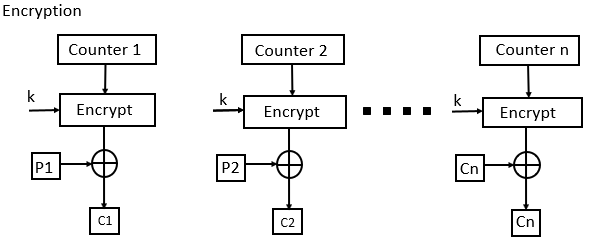
\includegraphics[width=0.5\textwidth]{KBE/img/ctr.png}
\end{figure}


\subsection{Cipher block chaining (CBC)}

Ciphertext se xoruje s plaintextem následujícího bloku, pak se to celé šifruje. Problém je, že na konci v posledním ciphertextu bude padding. A pokud správně správu zarovnáme, tak můžeme na konci kontrolovat padding.

Vezmeme ciphertext, který chceme rozklíčovat, a zjistíme, ve kterém bloku jsou data, která nás zajímají. Pak zahodíme vše, co je za nimi. Pak budeme manipulovat s posledním bytem předposledního bloku (ciphertext předposledního bloku se xoruje s plaintextem), a zkoušet posílat takový ciphertext na server. Při dešifrování vyjdou serveru v předposledním bloku kraviny, ale to nás nezajímá. Pokud na posledním místě posledního bloku bude 0x01, je to platný padding, jinak server hodí chybu.

Pokud chybu nehodí, víme, že xor posledních bytů v ciphertextu předposledního bloku a plaintextu paddingu (tedy 0x01) nám dá plaintext posledního bloku - to je to, co jsme chtěli zjistit.

Pak upravíme poslední byte předposledního bloku tak, aby nám vycházelo po xoru 0x02, a budeme měnit předposlední byte, dokud to neprojde - to znamená, že server přijal padding (0x02, 0x02), a tím získáme další byte.


\subsection{Galois counter mode - GCM}

GCM zároveň šifruje a podepisuje, používá transformace na Galoisových tělesech. Nevýhodou je, že autenticita je potvrzena až na konci přenosu (což se nehodí, třeba když chceme streamovat video). Je to jediné schéma v TLS1.3

\begin{figure}[ht!]
\centering
\begin{minipage}{.5\textwidth}
  \centering
  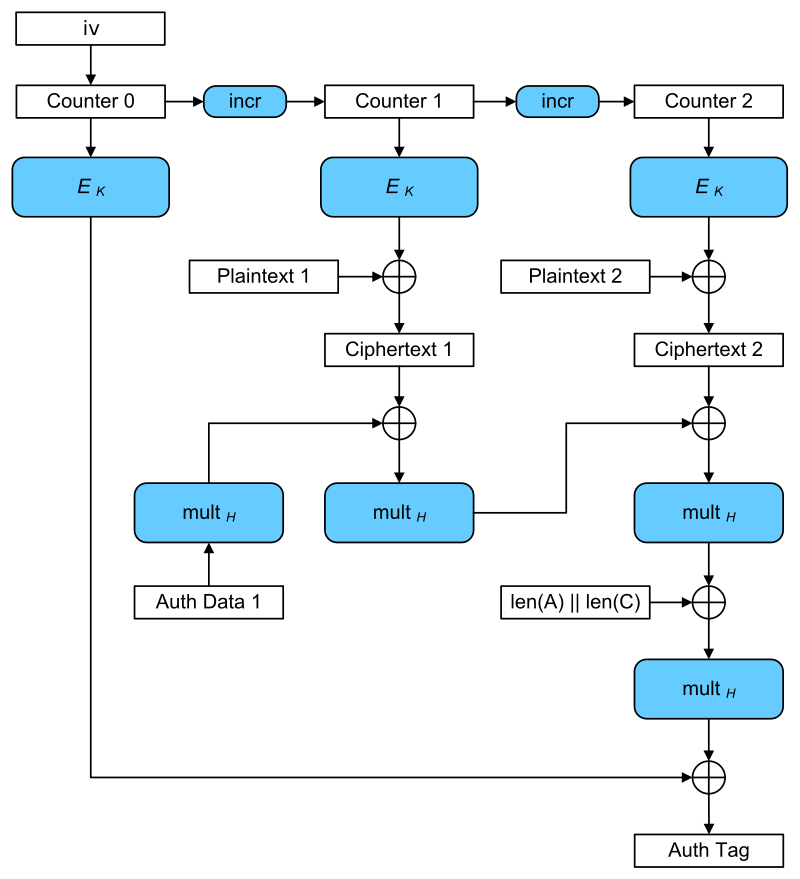
\includegraphics[width=\linewidth]{KBE/img/gcm.png}
  \caption{GCM pro blokové šifry}
  \label{fig:test1}
\end{minipage}%
\begin{minipage}{.5\textwidth}
  \centering
  \includegraphics[width=\linewidth]{KBE/img/needham-schroeder.png}
  \caption{Needham Schroederova výměna klíče}
  \label{fig:test2}
\end{minipage}
\end{figure}


\section{Needham-Schroederova výměna klíče}

DH, El Gamal, RSA a podobně jsou rozepsané v MKR, takže tady ukážu jen Needham-Shroederovu výměnu klíče, která je základem pro Kerberos. NS využívá toho, že obě strany důvěřují nějakému serveru. Každý účastník má vlastní klíč (symetrický), a jeho kopie je uložená na serveru. Alice, která chce komunikovat s Bobem, pošle serveru žádost, a server odpoví zašifrovaně (aby to nemohl přečíst nikdo jiný než Alice), a pošle v tom i klíč SK a token pro Boba. Alice pošle Bobovi token, ten je ho schopný dešifrovat svým klíčem, a pak jsou schopni komunikovat pomocí klíče SK.

Nevýhodou je, že tokeny posílané Bobovi platí věčně, není tam žádná kontrola času. Odcházející pracovník banky (Alice) si může vygenerovat několik set tokenů, uložit si je a Bob nemůže vědět, že Alice už v bance nepracuje. Dnes to je problém, ale v době vzniku NS protokolu byly počítače halové a bylo jich málo.





\section{Bitcoin a jiné měny}

\subsection{Vznik peněz}
Peníze se prvně objevily ve staré Číně nebo v Mezopotámii 2k př. n. l. Ohledně vzniku peněz jsou dvě teorie. První z nich říká, že některá z obchodovaných komodit se stala natolik významnou, že se stala použitelnou jako platidlo. Druhá teorie říká, že peníze vznikly společně s vypalovanými destičkami. Ty totiž mohly obsahovat ověřené (zapečetěné) sliby, směnky, dluhy, a tedy příslib platby. Přirozeně se pak příslib platby mohl přesunout někomu jinému.

Často byly penězi mince, které vydávala mincovna řízená panovníkem. Mince byly ražené, aby zajistily integritu. I přesto se ale s mincemi manipulovalo - lidé je ořezávali a ze získaného kovu odlévali nové mince. Mincovny v době krize šidily odlévaný kov a přidávaly do něj levnější příměsi.

\subsection{Inflace}
Moderní peníze vydávané centrálními bankami podléhají inflaci, tedy znehodnocení. To je dané tím, že objem peněz v oběhu se stále zvětšuje, jednak tiskem nových peněz, jednak půjčkami jiným bankám. Za stejný objem peněz se tedy s postupujícím časem dá koupit méně a méně zboží.

U kryptoměn se inflace nevyskytuje, protože jsou navrženy tak, aby nešly vydávat další peníze.

\subsection{Kryptoměny jako směnky}

Kryptoměny jsou založené na shodě komunity spíš než na centrální autoritě. Vypadají podobně jako směnky ze středověké Francie: \textit{Já, X, slibuji zaplatit částku Y panu Z.}

Při obchodování mohl pan Z zaplatit směnkou panu W, pokud pan W věřil tomu, že X peníze splatí. Na směnku se pak připisovali noví vlastníci. Po zaplacení byla směnka zničena. \textit{Já, Z, si přeji, aby peníze byly vyplaceny panu W.}

Obdobně v kryptoměnách vzniká blockchain, což je vlastně sekvence plateb a závazků. Kryptoměny jsou směnky, lze je dělit a dávat někomu jinému (platit).

\subsection{Eliptické křivky pro podpisy}

Pro výpočet podpisu je dán veřejný klíč $a, b, p, G, N$, kde $a, b$ jsou parametry křivky, ze které vznikla grupa, $p$ je modul, $G$ je generátor a $N$ je počet prvků v grupě (bodů na křivce).

Zvolíme náhodný soukromý klíč $d_a$ (v bitcoinu má 256bitů), a spočítáme veřejný klíč $Q_a$ jako opakované přičítání generátoru: $Q_a = d_a * G$. To je podobné jako v DSA, kde se počítalo $g^{d_a}$. Všechno počítání probíhá v modulu $p$.

Pak pro podepsání zprávy z hashem $m$ vygenerujeme nonce $k$. Spočítáme $P = k * G$, a přečteme $R$ jako x-ovou souřadnici bodu $P$. Pak podpis je $s$: $s = (m + d_a * R) * k^{-1}$.

Adresátovi se pak posílá zpráva s příslušným hashem, veřejné parametry $(a, b, p, G, N)$, klíč $Q_a$.
TODO

Při verifikaci se spočítá $P = s^{-1} * m * G + s^{-1} * R * Q_a$.

\paragraph{Důkaz správnosti}
$
P = s^{-1} m G + s^{-1} R Q_a
P = s^{-1} m G + s^{-1} R d_a G
P = s^{-1} G m + s^{-1} G R d_a
P = s^{-1} G (m + R d_a)
k = s^{-1} (m + R d_a)$

\subsection{EC a Bitcoin}

hash $Q_a$ je adresa peněženky
transakce má na vstupu předchozí transakce
na výstupu jsou transakce a poplatek

Blockchain se skládá z bloků, blok je sbírka transakcí (merkelovy stromy). Každý blok obsahuje hash předchozího bloku, tím jsou seřazeny jasně za sebe.

Další článek do bloku přidávají mineři, kteří sbírají transakce do bloku a pak se snaží najít hodnotu, která s hashem poslendího uzavřeného bloku vyjde "nějak hezky". Ten miner, kterému se to podaří nejrychleji, přidá za blockchain nový blok, a ostatní mineři nově začnou počítat s tímto blokem. Ten, kdo blok uzavře, dostane odměnu z poplatků transakcí.


